\documentclass[10pt]{article}
\usepackage[russian]{babel}
\usepackage[utf8]{inputenc}
\usepackage[T2A]{fontenc}
\usepackage{amsmath}
\usepackage{amsfonts}
\usepackage{amssymb}
\usepackage[version=4]{mhchem}
\usepackage{stmaryrd}
\usepackage{graphicx}
\usepackage[export]{adjustbox}
\graphicspath{ {./images/} }

\begin{document}
\section*{Нелинейный резонанс}
Как известно, для линейного осциллятора характерен эффект резонанса. Когда частота воздействия близка к собственной частоте осциллятора, амплитуда колебаний оказывается большой. Действительно, решение уравнения для вынужденных колебаний линейного осциллятора


\begin{equation*}
\ddot{x}+\omega_{0}^{2} x=f \cos \omega t \tag{14.6}
\end{equation*}


можно искать в виде $x=A \cos \omega t$. Подстановка этого выражения в уравнение приводит к соотношению


\begin{equation*}
|A|=\frac{f}{\left|\omega^{2}-\omega_{0}^{2}\right|}, \tag{14.7}
\end{equation*}


откуда следует, что при приближении частоты воздействия $\omega$ к собственной частоте $\omega_{0}$ амплитуда колебаний стремится к бесконечности (если учитывать диссипацию, она оказывается ограниченной).

В случае нелинейного осциллятора частота свободных колебаний обычно зависит от амплитуды (неизохронность). Например, для кубического осциллятора


\begin{equation*}
\ddot{x}+\omega_{0}^{2} x+\beta x^{3}=0 \tag{14.8}
\end{equation*}


колебания малой амплитуды, которые еще можно приближенно считать гармоническими, $x=A \cos \omega t$, происходят на частоте, сдвинутой на величину $\Delta \omega(A) \approx 3 \beta A^{2} / 8 \omega_{0}$ (см. лекцию 9).

В грубом приближении для описания вынужденных колебаний нелинейного осциллятора мы можем попытаться использовать то же самое соотношение (14.7), но вместо $\omega_{0}$ подставить модифицированную частоту свободных колебаний $\omega_{0}+\Delta \omega(A)$. В результате получается неявное соотношение, связывающее амплитуду вынужденных колебаний $A$ с частотой $\omega$ и амплитудой $f$ внешнего воздействия:


\begin{equation*}
|A|=\frac{f}{\left|\omega^{2}-\left(\omega_{0}+\Delta \omega\right)^{2}\right|} \approx \frac{f}{\left|\omega^{2}-\omega_{0}^{2}-3 \beta A^{2} \omega_{0}^{2} / 4\right|} . \tag{14.9}
\end{equation*}


На рис. 14.4 показаны графики зависимости амплитуды вынужденных колебаний от частоты для линейного (a) и нелинейного (б, в) осциллятора. Обратим внимание на разное расположение резонансной кривой осциллятора с кубической нелинейностью при положительном и отрицательном значении параметра нелинейности $\beta$. Если частота свободных колебаний возрастает с ростом амплитуды (при $\beta>0$ ), то верхняя часть графика резонансной кривой наклонена вправо, если же убывает (при $\beta<0$ ), то влево.

Следует отметить, что в отличие от линейного случая амплитуда вынужденных колебаний остается конечной даже при точном совпадении $\omega$ и $\omega_{0}$. Причина, очевидно, заключается в неизохронности собственных колебаний нелинейного осциллятора: с ростом амплитуды увеличивается нелинейный сдвиг частоты и резонансные условия нарушаются. Вследствие этого нарастание амплитуды ограничивается.

Совокупность явлений, которые наблюдаются в нелинейном осцилляторе при внешнем периодическом воздействии и проявляются в изменении качественной природы и количественных характеристик вынужденных колебаний в зависимости от амплитуды и частоты воздействия, обозначают термином нелинейный резонанс. Важно подчеркнуть, что зависимость амплитуды от частоты, как видно из рис. 14.4, может быть

неоднозначной. Это очень существенный и характерный для нелинейного резонанса момент, который будет подробнее обсужден в ходе дальнейшего изложения.\\
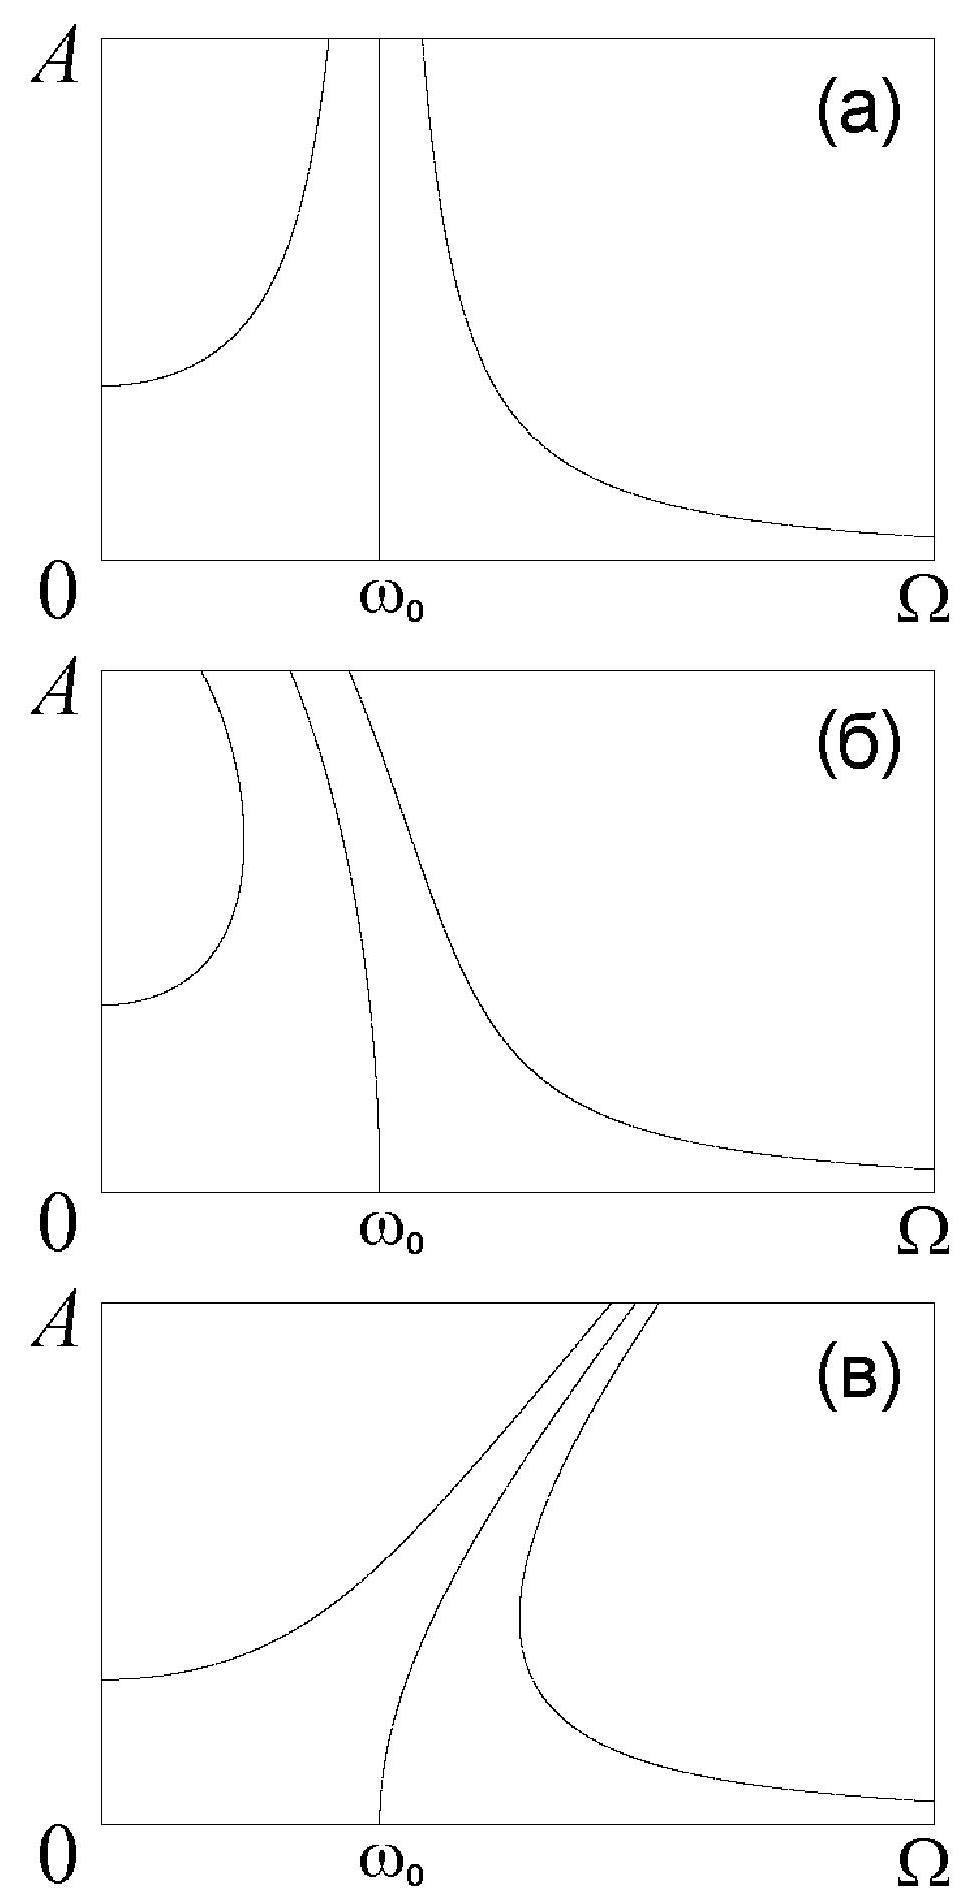
\includegraphics[max width=\textwidth, center]{2024_12_13_cd59585e7886a9efee75g-219}

Рис. 14.4. Резонансные кривые - зависимость амплитуды вынужденных колебаний от частоты воздействия в линейном осцилляторе (a) и в нелинейном осцилляторе с кубической нелинейностью при $\beta<0$ (б) и $\beta>0$ (в) в отсутствие диссипации.

Резонансные кривые для консервативного осциллятора можно встретить в многочисленных учебных курсах по теории колебаний. Правильная их интерпретация со-

держит определенную тонкость, что не всегда должным образом подчеркивается. Дело в том, что консервативный осциллятор (как линейный, так и нелинейный) обладает свойством сохранять «память» о своем начальном состоянии на протяжении неограниченного времени. Поэтому в общем случае движение будет содержать зависящую от начальных условий составляющую, отвечающую за «собственные» колебания осциллятора с некоторой характерной частотой и амплитудой, и составляющую, отвечающую за вынужденные колебания, период которой определяется периодом воздействия (в нелинейной системе принцип суперпозиции не работает, поэтому, говоря о наличии двух составляющих колебательного процесса, мы имеем в виду не их сумму, а некую более сложную комбинацию). Если частоты обеих составляющих находятся в рациональном отношении, то движение будет периодическим, но это скорее исключительный случай. Если же частоты несоизмеримы, то движение оказывается квазипериодическим. Только лишь при определенном выборе начальных условий, исключающим «собственную» колебательную составляющую, реализуются «в чистом виде» вынужденные колебания, которым соответствует амплитуда, представленная на рис.14.4.

Можно, однако, предложить и другой подход к трактовке резонансных кривых на рис.14.4. Представим себе, что наш осциллятор на самом деле диссипативный, но диссипация исчезающе мала (характеризуется параметром $\gamma<<1$ ). Тем не менее, если время наблюдения достаточно велико, $T \gg \gamma^{-1}$, то диссипация будет существенной и обеспечит установление не зависящего от начальных условий режима вынужденных колебаний. Зависимость амплитуды колебаний от частоты воздействия в установившемся режиме будет приближенно описываться резонансными кривыми, построенными для консервативного осциллятора, с тем большей точностью, чем меньше параметр диссипации $\alpha$.

\end{document}